\chapter{Proposed Solution}

\begin{chapquote}{Jim Barksdale}
If we have data, let’s look at data. If all we have are opinions, let’s go with mine.
\end{chapquote}

\section{Introduction}

Perform a data driven analysis required to develop a collection of tools
that are good enough to run in a lightning network node with daly activity. 
In this section is described an open source framework for the definition and 
the collection of lightning network metrics.

Therefore, in order to implement this framework, and analysis of the state 
of the art was required (descibed in the Section \ref{sec:problem_and_state_of_the_art})
to better understanding what are the information that are more difficult 
to get from a researcher point of view.

From our preliminary study we found that information on how a node perform 
on a daily basis are difficult to get, due the following problems:
\begin{itemize}
    \item Requires a direct interaction with the\emph{node operators};\footnote{node operators are people that own a lightning node that point to 
    help the network in routing payments.}
    \item Data collection of this kind can lend of some
    that a node operators may want not share.
\end{itemize}

So, in order to work around to these problem our proposal is define in a 
public manner what data will be collected, and how these are analyzed. This 
definition process is done through a lnmetrics Request for Comments (RFC) 
called \emph{lnmetrics RFC}. Then, after the data are defined, the collection 
of this data is done with a public server with public API with the possibility 
to self hosting the server on hardwar with at least of a Raspberry PI 2 capability.

In addition, in order to incentivize the node operators to provide share the 
information with one of the public server available we write the tool that 
collect the information on the lightning node with the possibility to ran 
in an offline mode, and only if and when the node operators want the data 
are shared with one of the server choosed (or more than one server).

The Figure \ref{fig:lnmetrics_process} shows as the general process of propose a solution that 
required daily data analysis to solve a problem looks like.

\begin{figure}
    \begin{center}
      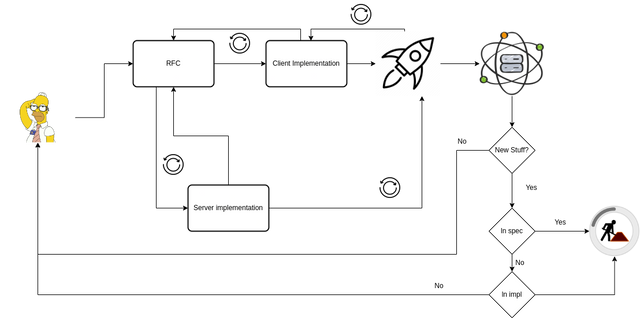
\includegraphics[scale=0.7]{imgs/lnmetrics-workflow-drawio.png}
    \end{center}
    \caption{Example of a process that use lnmetrics looks like.}
    \label{fig:lnmetrics_process}
\end{figure}


\section{LNMetrics Request for Comments (RFC)}

The LNMetics Request for Comment (RFC) proposed is a more general idea of what 
it is already done in the Lightning Network protocol definition. In fact,
this RFC is point to have the data description of what data are collected in 
order and how these data are used. It is not trying to define an only way to 
define a particular metrics on the lightning nertwork, but more to incentivize
discussion between people to achive a better result.
